In this project, mapping and localization are closely linked together. In order to create a map, the current location of the \acs{uav} in its area has to be known to be used as a reference point. However, to get the current location of the \acs{uav} in its area, the map of its area has to be known. Therefore, it can be described as a "chicken\hyp{}or\hyp{}egg" problem.

% https://medium.com/desn325-emergentdesign/s-l-a-m-tech-tracking-743d059b1468
This issue can be overcome through the usage of a pre-existing map of an environment, for example, \acs{gps} data. However, there is no data for an indoor environment and if there was, it would not be precise enough or updated in real\hyp{}time. Therefore, the introduction of a \acs{slam} algorithm which is capable of mapping and localizing simultaneously by using feature extraction.

% https://www.andreasjakl.com/basics-of-ar-slam-simultaneous-localization-and-mapping/
A \acs{slam} system consists of four parts: sensor data, a front\hyp{}end, a back\hyp{}end, and the \acs{slam} estimate. The sensor data is all the input data a \acs{slam} system receives. In the front\hyp{}end a feature extraction process is executed. These features are tracked through a stream of video in the back\hyp{}end. The back\hyp{}end also handles long\hyp{}term associations to reduce drift and triggers loop\hyp{}closures. As a result, the \acs{slam} systems outputs all tracked features with their locations and relations, as well as the position of the sensors within the world.

\begin{figure}[!h]
  \centering
  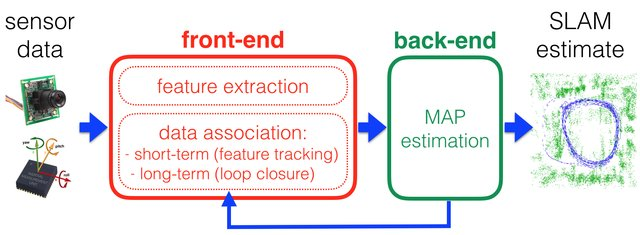
\includegraphics[width=0.75\linewidth]{images/slam_system.jpg}
  \caption{SLAM system}
  \label{fig:slam_system}
\end{figure}

% https://www.andreasjakl.com/basics-of-ar-anchors-keypoints-feature-detection/
As earlier mentioned, a \acs{slam} algorithm uses feature extraction as a way to track the movement of the \acs{uav} in space. The easiest way to explain how feature extraction works is its implementation on a camera. On every frame, features are detected. The way these features are detected differ from algorithm to algorithm. Every feature detected, needs a unique description based on its properties. 

The tracking of the features throughout the frames is handled in the back\hyp{}end. The descriptions of these features of different frames are compared. The motion of the \acs{uav} is based on the change of the position of these features relative to the previous frame. To keep account of moving objects and outliers, the majority of features must move in the same direction.

Not only the tracking of features is considered when estimating the motion of the \acs{uav}, but different sensor data influence the estimation. Most notable, the data from an accelerometer and a gyroscope. When the algorithm detects a frame it already has visited, it recalculates all previous locations to match this new finding. This is called a loop closure. With loop closures, a \acs{slam} algorithm updates previous values to keep the map as accurate and truthful as possible.